\documentclass[
  shownotes,
  xcolor={svgnames},
  hyperref={colorlinks,citecolor=DarkBlue,linkcolor=DarkRed,urlcolor=DarkBlue}
  , aspectratio=169]{beamer}
\usepackage{animate}
\usepackage{amsmath}
\usepackage{amsfonts}
\usepackage{amssymb}
\usepackage{pifont}
\usepackage{mathpazo}
%\usepackage{xcolor}
\usepackage{multimedia}
\usepackage{fancybox}
\usepackage[para]{threeparttable}
\usepackage{multirow}
\setcounter{MaxMatrixCols}{30}
\usepackage{subcaption}
\usepackage{graphicx}
\usepackage{lscape}
\usepackage[compatibility=false,font=small]{caption}
\usepackage{booktabs}
\usepackage{ragged2e}
\usepackage{chronosys}
\usepackage{appendixnumberbeamer}
\usepackage{animate}
\setbeamertemplate{caption}[numbered]
\usepackage{color}
%\usepackage{times}
\usepackage{tikz}
\usepackage{comment} %to comment
%% BibTeX settings
\usepackage{natbib}
\bibliographystyle{apalike}
\bibpunct{(}{)}{,}{a}{,}{,}
\setbeamertemplate{bibliography item}{[\theenumiv]}

% Defines columns for bespoke tables
\usepackage{array}
\newcolumntype{L}[1]{>{\raggedright\let\newline\\\arraybackslash\hspace{0pt}}m{#1}}
\newcolumntype{C}[1]{>{\centering\let\newline\\\arraybackslash\hspace{0pt}}m{#1}}
\newcolumntype{R}[1]{>{\raggedleft\let\newline\\\arraybackslash\hspace{0pt}}m{#1}}


\usepackage{xfrac}


\usepackage{multicol}
\setlength{\columnsep}{0.5cm}

% Theme and colors
\usetheme{Boadilla}

% I use steel blue and a custom color palette. This defines it.
\definecolor{andesred}{HTML}{af2433}

% Other options
\providecommand{\U}[1]{\protect\rule{.1in}{.1in}}
\usefonttheme{serif}
\setbeamertemplate{itemize items}[default]
\setbeamertemplate{enumerate items}[square]
\setbeamertemplate{section in toc}[circle]

\makeatletter

\definecolor{mybackground}{HTML}{82CAFA}
\definecolor{myforeground}{HTML}{0000A0}

\setbeamercolor{normal text}{fg=black,bg=white}
\setbeamercolor{alerted text}{fg=red}
\setbeamercolor{example text}{fg=black}

\setbeamercolor{background canvas}{fg=myforeground, bg=white}
\setbeamercolor{background}{fg=myforeground, bg=mybackground}

\setbeamercolor{palette primary}{fg=black, bg=gray!30!white}
\setbeamercolor{palette secondary}{fg=black, bg=gray!20!white}
\setbeamercolor{palette tertiary}{fg=white, bg=andesred}

\setbeamercolor{frametitle}{fg=andesred}
\setbeamercolor{title}{fg=andesred}
\setbeamercolor{block title}{fg=andesred}
\setbeamercolor{itemize item}{fg=andesred}
\setbeamercolor{itemize subitem}{fg=andesred}
\setbeamercolor{itemize subsubitem}{fg=andesred}
\setbeamercolor{enumerate item}{fg=andesred}
\setbeamercolor{item projected}{bg=gray!30!white,fg=andesred}
\setbeamercolor{enumerate subitem}{fg=andesred}
\setbeamercolor{section number projected}{bg=gray!30!white,fg=andesred}
\setbeamercolor{section in toc}{fg=andesred}
\setbeamercolor{caption name}{fg=andesred}
\setbeamercolor{button}{bg=gray!30!white,fg=andesred}


\usepackage{fancyvrb}
\newcommand{\VerbBar}{|}
\newcommand{\VERB}{\Verb[commandchars=\\\{\}]}
\DefineVerbatimEnvironment{Highlighting}{Verbatim}{commandchars=\\\{\}}
% Add ',fontsize=\small' for more characters per line
\usepackage{framed}
\definecolor{shadecolor}{RGB}{248,248,248}
\newenvironment{Shaded}{\begin{snugshade}}{\end{snugshade}}
\newcommand{\AlertTok}[1]{\textcolor[rgb]{0.94,0.16,0.16}{#1}}
\newcommand{\AnnotationTok}[1]{\textcolor[rgb]{0.56,0.35,0.01}{\textbf{\textit{#1}}}}
\newcommand{\AttributeTok}[1]{\textcolor[rgb]{0.77,0.63,0.00}{#1}}
\newcommand{\BaseNTok}[1]{\textcolor[rgb]{0.00,0.00,0.81}{#1}}
\newcommand{\BuiltInTok}[1]{#1}
\newcommand{\CharTok}[1]{\textcolor[rgb]{0.31,0.60,0.02}{#1}}
\newcommand{\CommentTok}[1]{\textcolor[rgb]{0.56,0.35,0.01}{\textit{#1}}}
\newcommand{\CommentVarTok}[1]{\textcolor[rgb]{0.56,0.35,0.01}{\textbf{\textit{#1}}}}
\newcommand{\ConstantTok}[1]{\textcolor[rgb]{0.00,0.00,0.00}{#1}}
\newcommand{\ControlFlowTok}[1]{\textcolor[rgb]{0.13,0.29,0.53}{\textbf{#1}}}
\newcommand{\DataTypeTok}[1]{\textcolor[rgb]{0.13,0.29,0.53}{#1}}
\newcommand{\DecValTok}[1]{\textcolor[rgb]{0.00,0.00,0.81}{#1}}
\newcommand{\DocumentationTok}[1]{\textcolor[rgb]{0.56,0.35,0.01}{\textbf{\textit{#1}}}}
\newcommand{\ErrorTok}[1]{\textcolor[rgb]{0.64,0.00,0.00}{\textbf{#1}}}
\newcommand{\ExtensionTok}[1]{#1}
\newcommand{\FloatTok}[1]{\textcolor[rgb]{0.00,0.00,0.81}{#1}}
\newcommand{\FunctionTok}[1]{\textcolor[rgb]{0.00,0.00,0.00}{#1}}
\newcommand{\ImportTok}[1]{#1}
\newcommand{\InformationTok}[1]{\textcolor[rgb]{0.56,0.35,0.01}{\textbf{\textit{#1}}}}
\newcommand{\KeywordTok}[1]{\textcolor[rgb]{0.13,0.29,0.53}{\textbf{#1}}}
\newcommand{\NormalTok}[1]{#1}
\newcommand{\OperatorTok}[1]{\textcolor[rgb]{0.81,0.36,0.00}{\textbf{#1}}}
\newcommand{\OtherTok}[1]{\textcolor[rgb]{0.56,0.35,0.01}{#1}}
\newcommand{\PreprocessorTok}[1]{\textcolor[rgb]{0.56,0.35,0.01}{\textit{#1}}}
\newcommand{\RegionMarkerTok}[1]{#1}
\newcommand{\SpecialCharTok}[1]{\textcolor[rgb]{0.00,0.00,0.00}{#1}}
\newcommand{\SpecialStringTok}[1]{\textcolor[rgb]{0.31,0.60,0.02}{#1}}
\newcommand{\StringTok}[1]{\textcolor[rgb]{0.31,0.60,0.02}{#1}}
\newcommand{\VariableTok}[1]{\textcolor[rgb]{0.00,0.00,0.00}{#1}}
\newcommand{\VerbatimStringTok}[1]{\textcolor[rgb]{0.31,0.60,0.02}{#1}}
\newcommand{\WarningTok}[1]{\textcolor[rgb]{0.56,0.35,0.01}{\textbf{\textit{#1}}}}
\usepackage{graphicx}
\makeatletter

\makeatother






%%%%%%%%%%%%%%% BEGINS DOCUMENT %%%%%%%%%%%%%%%%%%

\begin{document}

\title[Lecture 6]{Lecture 6: \\ MLE \\ Intro To Scraping}
\subtitle{Big Data and Machine Learning for Applied Economics \\ Econ 4676}
\date{\today}

\author[Sarmiento-Barbieri]{Ignacio Sarmiento-Barbieri}
\institute[Uniandes]{Universidad de los Andes}


\begin{frame}[noframenumbering]
\maketitle
\end{frame}

%%%%%%%%%%%%%%%%%%%%%%%%%%%%%%%%%%%



%----------------------------------------------------------------------%
\begin{frame}
\frametitle{Recap}

\begin{itemize} 
  
    \item Least Square Estimator
    \medskip
    \item Problem Set    
    \medskip
    \item Github Repos
    \medskip
    \item Bonus: Contribuir con los tutorials ya sea en  \texttt{Python}  o \texttt{R}:  0.25 bonus de la nota final (max 1 punto)

\end{itemize}

\end{frame}

%----------------------------------------------------------------------%

\begin{frame}
\frametitle{Agenda}

\tableofcontents


\end{frame}



%----------------------------------------------------------------------%
\section{Motivation}
%----------------------------------------------------------------------%
\begin{frame}[fragile]
\frametitle{Motivation}

\begin{itemize}
    \item Maximum Likelihood is, by far, the most popular technique for deriving estimators
    \bigskip 
    \item Developed by Ronald A. Fisher (1890-1962)
    \bigskip
    \item ``If Fisher had lived in the era of ``apps,'' maximum likelihood estimation might have made him a billionaire'' (Efron and Tibshiriani, 2016)
    \bigskip
    \item  Why? MLE gives ``automatically''
    \begin{itemize}
      \item Unbiasedness 
      \medskip
      \item Minimum variance
    \end{itemize} 
\end{itemize}
 


 \end{frame}
%----------------------------------------------------------------------%
\section{Maximum Likelihood Estimation}
%----------------------------------------------------------------------%
\begin{frame}[fragile]
\frametitle{Maximum Likelihood Estimation vs Density}
\begin{itemize}
\item Let $X$ be a random variable with density $f(x,\theta)$ 
\medskip
\item And $X_1,\dots,X_n$ and iid sample $\sim_{iid}f(x|\theta)$
\medskip
\item The likelihood function for $X$ is
\medskip
\begin{align}
\mathcal{L}(\theta|x):\mathbb{R}^K \rightarrow \mathbb{R}
\end{align}
\item Note the following,
\medskip
\begin{enumerate}
  \item In the density function, $\theta$ is taken as given, and $x$ varies
  \medskip
  \item In the likelihood function, $x$ is taken as given, and $\theta$ varies
\end{enumerate}
\end{itemize}

 \end{frame}
%----------------------------------------------------------------------%
\begin{frame}[fragile]
\frametitle{Maximum Likelihood Estimation}
\framesubtitle{Example}

\begin{itemize}
\item Let $X\sim N(\mu,\sigma^2)$
\medskip
\item Note that $
 \theta=\left(\begin{array}{c}
 \mu\\
 \sigma^{2}
 \end{array}\right)$
\medskip
 \item Then 
 \medskip
   \begin{itemize}
     \item  $f(x|\theta) : \mathbb{R}\rightarrow  \mathbb{R}$ and $f(x,\theta)=\frac{1}{\sqrt{2\pi\sigma^{2}}}exp\left(- \frac{(x-\mu)^2}{2\sigma^2} \right)$
     \medskip
     \item  $ \mathcal{L}(\theta|x) : \mathbb{R}^2 \rightarrow  \mathbb{R}$ and  $\mathcal{L}(\theta|x) =\frac{1}{\sqrt{2\pi\sigma^{2}}}exp\left(- \frac{(x-\mu)^2}{2\sigma^2} \right)$
   \end{itemize}
\medskip
   \item Intuition?
\end{itemize}

\end{frame}
%----------------------------------------------------------------------%


\begin{frame}[fragile]
\frametitle{Maximum Likelihood Estimation}

Let $X_1,\dots,X_n\sim_{iid}f(x|\theta)$, the likelihood function is defined by

\begin{align}\label{eq:1}
\mathcal{L}(\theta|x)=\Pi_{i=1}^n \mathcal{L_{i}}(\theta|x)=\Pi_{i=1}^n f(x_i|\theta)
\end{align}

A maximum likelihood estimator of the parameter $\theta$:

\begin{align}
\hat \theta^{MLE}=\underset{\theta \in \Theta}{argmax}\, \mathcal{L}(\theta|x)
\end{align}


\end{frame}
%----------------------------------------------------------------------%

\begin{frame}[fragile]
\frametitle{Maximum Likelihood Estimation}

\begin{itemize}
  \item Intuitively, MLE is a reasonable choice for an estimator.
  \medskip
  \item MLE is the parameter point for which the observed sample is most likely
  \medskip
  \item {\it It is kind of a ‘reverse engineering’ process:  to generate random numbers for a certain distribution you first set parameter values and then get realizations. This is doing the reverse process:  first set the realizations and try to get the parameters that are ‘most likely’ to have generated them}
\end{itemize}


 \end{frame}
%----------------------------------------------------------------------%

\begin{frame}[fragile]
\frametitle{Maximum Likelihood Estimation}
Note that maximizing 

\begin{align}\label{eq:1}
\mathcal{L}(\theta|x)=\Pi_{i=1}^n f(x_i|\theta)
\end{align}

is the same as maximizing

\begin{align}\label{eq:2}
l(\theta|x)=\ln \mathcal{L}(\theta|x)=\sum_{i=1}^n l_i(x|\theta)
\end{align}

\bigskip
Advantages of \eqref{eq:2}
\begin{itemize}
\item It is easy to see that the {\bf contribution} of observation $i$ to the likelihood is given by $l_i(x|\theta)=\ln f(x_i|\theta)$
\item Eq. \eqref{eq:1} is also prone to underflow; can be very large or very small number that it cannot easily be represented in a computer. 
\end{itemize}

\end{frame}

%----------------------------------------------------------------------% 

\begin{frame}[fragile]
\frametitle{Maximum Likelihood Estimation}
If the likelihood function is differentiable (in $\theta$) a possible candidate for the MLE are the values of $\theta$ that solve

\begin{align}
  \frac{\partial \mathcal{L}(\theta|x)}{\partial \theta} = 0
\end{align}

\begin{itemize}
\item These are  only {\it possible candidates}, this is a necessary condition for a max
\item Need to check SOC
\end{itemize}

\end{frame}
%----------------------------------------------------------------------%

\begin{frame}[fragile]
\frametitle{Maximum Likelihood Estimation}

 Let $X_1,\dots,X_n \sim_{iid} N(\mu,1)$. We want to estimate $\theta = \mu$

Here

\begin{align}
l(\theta |x)=\frac{1}{(\sqrt{2\pi})^{n}}e^{-\frac{1}{2}\sum_{i=1}^{n}(x_i-\mu)^2}
\end{align}


taking logs 

\begin{align}
l\left(\theta |x\right)=-\frac{n}{2}log\left(2\pi\right)-\frac{1}{2}\sum_{i=1}^{n}(x_i-\mu)^2
\end{align}

FOC

\begin{align}
\frac{\partial l\left(\theta |x\right)}{\partial\mu}=0
\end{align}


\end{frame}
%----------------------------------------------------------------------%

\begin{frame}[fragile]
\frametitle{Maximum Likelihood Estimation}

\begin{align}
\frac{\partial l\left(\theta |x\right)}{\partial\mu}=2\frac{\sum_{i=1}^{n}\left(x_{i}-\mu\right)}{2}=0
\end{align}


\begin{align}
\sum_{i=1}^{n}\left(x_{i}-\hat{\mu}\right)=0
\end{align}

then

\begin{align}
\hat{\mu}=\frac{\sum_{i=1}^{n}x_{i}}{n}=\bar{x}
\end{align}

The MLE is the sample mean. Next we check the SOC


\begin{align}
\frac{\partial^2l(\theta|x)}{\partial \theta^2}=-n<0
\end{align}

We are in  a global maximum

\end{frame}
%----------------------------------------------------------------------%
\section{Profile Likelihood }
%----------------------------------------------------------------------%
\begin{frame}[fragile]
\frametitle{Concentrated/Profile Likelihood }

Suppose now, that $f(y,x|\eta)$ is the joint density function of two variables $X$ and $Y$.  Then, it can be decomposed as

\begin{align}
f(y,x|\eta) =f(y|x,\theta)f(x|\phi)
\end{align}

\begin{itemize}
  \item $\theta,\,\phi \subset \eta$ 
  \medskip
  \item The parameter vector of interest is  $\theta$ and $\theta$ and $\phi$ are functionally unrelated
  \medskip
  \item Maximizing the joint likelihood is achieved through maximizing separately the conditional and the marginal likelihood
  \medskip
  \item The MLE of $\theta$ also maximizes the conditional likelihood  
  \medskip
  \item We can obtain ML estimates by specifying the conditional likelihood only, reducing computational burden of the original problems
\end{itemize}  
\end{frame}

%----------------------------------------------------------------------%
\section{Example}
%----------------------------------------------------------------------%
\begin{frame}[fragile]
\frametitle{Example 1: Linear Regression}

Now consider the following linear model 
\medskip

\begin{align}
y=X\beta+u \\
u\sim_{iid} N(0,\sigma^2I)
\end{align}

\medskip
Note that $y_i|X_i\sim N(X_i\beta,\sigma^2)$ thus the pdf of $y_i|X$
\medskip
\begin{align}
f_i(y_i|\beta,\sigma,X_i)=\frac{1}{(\sqrt{2\pi\sigma^2})}e^{-\frac{1}{2\sigma^2}(y_i-X_i\beta)^2}
\end{align}


\end{frame}

%----------------------------------------------------------------------%
\begin{frame}[fragile]
\frametitle{Example 1: Linear Regression}
The contribution to the log likelihood from observation $i$

\begin{align}
l_i(y_i|\beta,\sigma,X_i)=-\frac{1}{2}log 2 \pi-\frac{1}{2}log\sigma^2-\frac{1}{2\sigma^2}(y_i-X_i\beta)^2
\end{align}

Since we assumed that obs are $iid$, then the log likelihood

\begin{align}
l(y|\beta,\sigma,X) &=-\frac{n}{2}log 2 \pi-\frac{n}{2}log\sigma^2-\frac{1}{2\sigma^2}\sum_{i=1}^n(y_i-X_i\beta)^2  \\
&=-\frac{n}{2}log 2 \pi-\frac{n}{2}log\sigma^2-\frac{1}{2\sigma^2}(y-X\beta)'(y-X\beta)
\end{align}
The ML estimators for $\beta$ and $\sigma$ result from maximizing this last line

\end{frame}
%----------------------------------------------------------------------%
\begin{frame}[fragile]
\frametitle{Example 1: Linear Regression}


The first step in maximizing $l(y|\beta,\sigma,X)$ is to {\bf concentrate} it with respect to $\sigma$

\begin{align}
\frac{\partial l}{\partial \sigma}&=-\frac{n}{2\sigma}+\frac{1}{\sigma^3}(y-X\beta)'(y-X\beta)=0
\end{align}

Solving for $\sigma^2$

\begin{align}
\hat \sigma^2(\beta) = \frac{1}{n}(y-X\beta)'(y-X\beta)
\end{align}

\end{frame}


%----------------------------------------------------------------------%
\begin{frame}[fragile]
\frametitle{Example 1: Linear Regression}

Replacing this in the log likelihood we get the concentrated (profile) likelihood

\begin{align}
l^c(y|\beta,X) = -\frac{n}{2}log 2 \pi-\frac{n}{2}log\left( \frac{1}{n}(y-X\beta)'(y-X\beta)\right)-\frac{n}{2}
\end{align}

\medskip

\begin{enumerate}
 \item Get $\hat \beta$
 \item Replace $\beta$ in $\hat \sigma^2(\beta) = \frac{1}{n}(y-X\beta)'(y-X\beta)$ $\rightarrow$ get $\hat \sigma^2$
\end{enumerate}

\medskip

This is not the only way, you could concentrate relative to $\beta$ first and solve for $\sigma^2$

\end{frame}
%----------------------------------------------------------------------%
\begin{frame}[fragile]
\frametitle{Example 2}

Let $y_i|X_i \sim_{iid} Bernoulli(p)$, where $p=Pr(y=1|X)=F(X\beta)$ and $F(.)$ normal cdf. Then the conditional likelihood is

\begin{align}
\mathcal{L}(\beta,Y)=\Pi_{i=1}^n p_i^{y_i}(1-p_i)^{1-y_i}
\end{align}
The log likelihood is then

\begin{align}
l(\beta,Y)=\sum_{i=1}^n\left(y_i \ln F(X_i\beta)+(1-y_i)\ln(1-F(X_i\beta))\right)
\end{align}

\end{frame}
%----------------------------------------------------------------------%
\begin{frame}[fragile]
\frametitle{Example 2}
FOC

\begin{align}
\frac{\partial l(\beta|y,X)}{\partial\beta}&=0 
\end{align}
\begin{align}
\overset{n}{\underset{i=1}{\sum}}y_{i}\frac{1}{F(X_{i}\beta)}f(X_{i}'\beta)X_{i}'+\overset{n}{\underset{i=1}{\sum}}\left(1-y_{i}\right)\frac{1}{\left(1-F(X_{i}'\beta)\right)}-f(X_{i}'\beta)X_{i}'&=0
\end{align}

\begin{centering}
$\vdots$
\end{centering}

\end{frame}
%----------------------------------------------------------------------%
\begin{frame}[fragile]
\frametitle{Example 2}
\begin{centering}
$\vdots$
\end{centering}

\begin{align}
\sum_{i=1}^n\frac{(y_i-F(X_{i}'\beta))f(X_{i}'\beta)x_i}{F(X_{i}'\beta)(1-F(X_{i}'\beta))}=0
\end{align}

\bigskip
Note:
\begin{itemize}
  \item This is a system of $K$ non linear equations with $K$ unknown parameters. 
  \item We cannot explicitly solve for $\hat \beta$
\end{itemize}


\end{frame}
%----------------------------------------------------------------------%
\section{Computation Newton-Method}
%----------------------------------------------------------------------%

\begin{frame}[fragile]
\frametitle{Computation Newton-Method}
\begin{itemize}
\item Here we can use Newton’s Method 
\end{itemize}
\bigskip
\begin{align}
    \theta'=\theta-H^{-1} \nabla_\theta f(\theta)
    \end{align}
\bigskip
\begin{itemize}
  \item Note the difference with Gradient Descent
  \medskip
  \item $H^{-1}$ should be negative definite, why? 
  %this ensures that the step will be in an uphill direction    
\end{itemize}

\end{frame}
%----------------------------------------------------------------------%

\begin{frame}[fragile]
\frametitle{Computation Newton-Method}
\begin{itemize}
\item Newton’s Method usually does not work well, when $H^{-1}$ is not n.d.
\medskip
\item Quasi-Newton Method
\end{itemize}

\begin{align}
    \theta'=\theta + \eta D^{-1} \nabla_\theta f(\theta)
    \end{align}

\begin{itemize}
  \item $\eta$ is an scalar determined at each step
  \medskip
  \item $D \approx -H$ so it's always positive definite
  \medskip
  \item When the loglikelihood function is globally concave and not too flat, maximizing it is usually quite easy. 
  \medskip
  \item When the loglikelihood function has several local maxima, doing so can be very difficult 
\end{itemize}

\end{frame}
%----------------------------------------------------------------------%
\section{Motiviation Web Scraping}
%----------------------------------------------------------------------%
\begin{frame}
\frametitle{Motiviation Web Scraping}



\begin{figure}[H] \centering
  \centering
  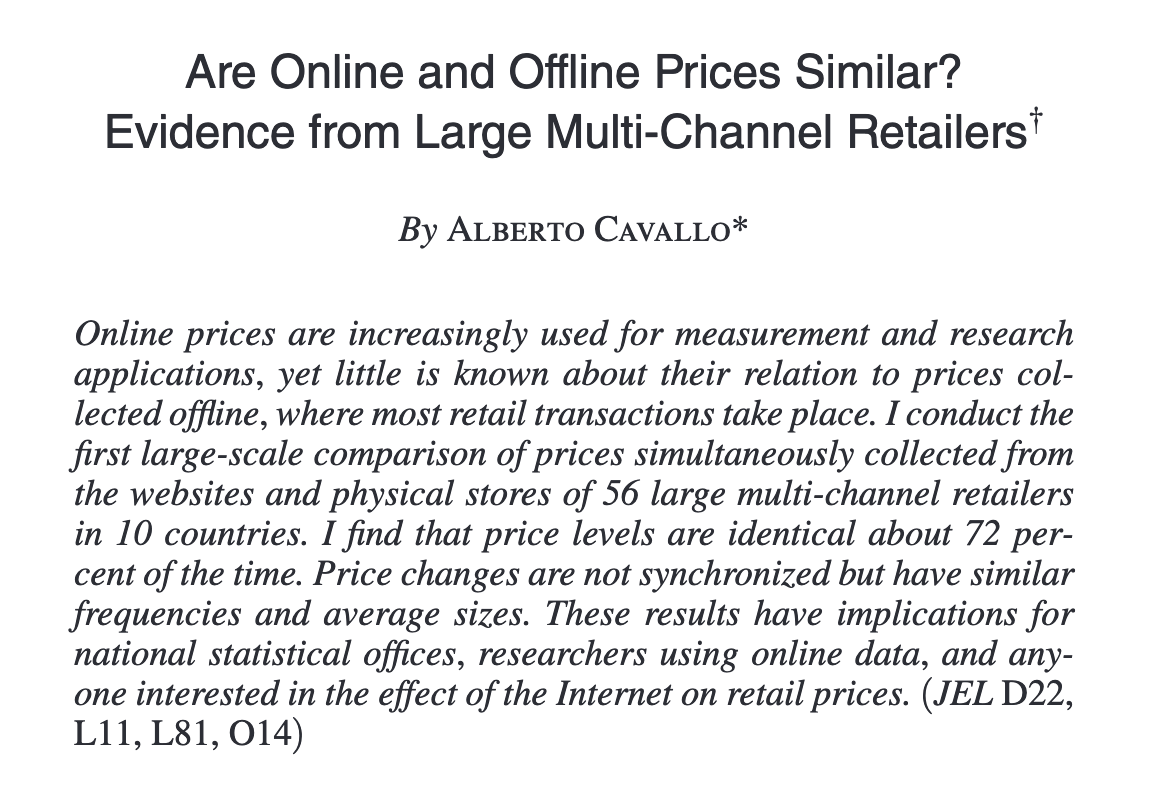
\includegraphics[scale=0.45]{figures/Cavallo_title}
  \\
  \tiny
\end{figure}
 

\end{frame}

%----------------------------------------------------------------------%
\begin{frame}
\frametitle{Motiviation Webscraping}



\begin{figure}[H] \centering
  \centering
  
\includegraphics[scale=0.25]{figures/Cunningham_title}
  \\
  \tiny
\end{figure}
 

\end{frame}

%----------------------------------------------------------------------%

\begin{frame}
\frametitle{Motiviation Webscraping}



\begin{figure}[H] \centering
  \centering
  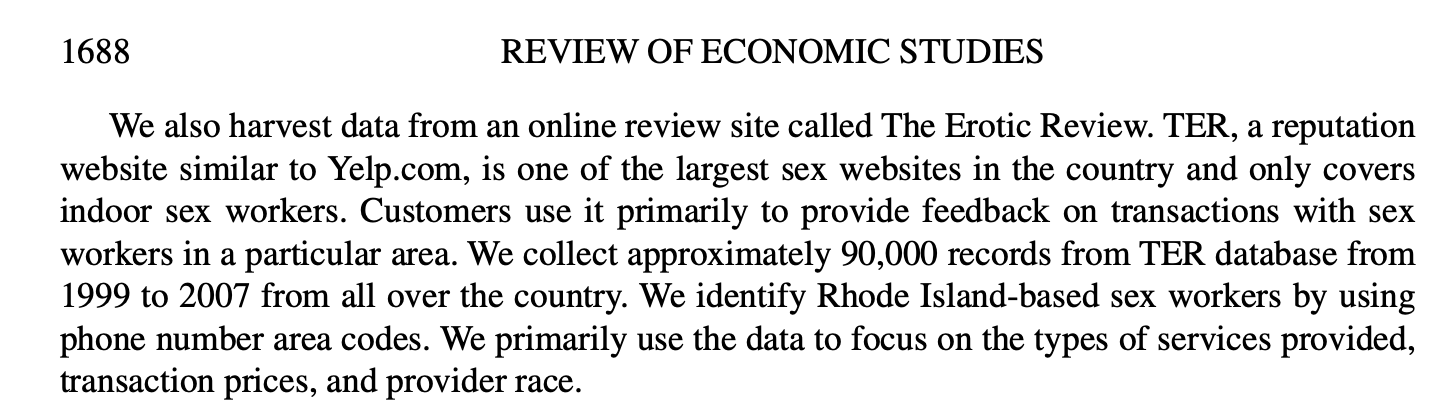
\includegraphics[scale=0.45]{figures/Cunningham_desc}
  \\
  \tiny
\end{figure}
 

\end{frame}


%----------------------------------------------------------------------%

\begin{frame}
\frametitle{Webscraping basics}

\begin{figure}[H] \centering
  \centering
  
\includegraphics[scale=0.75]{figures/webscrape_it.jpg}
  \\
  \tiny
\end{figure}

\end{frame}

%----------------------------------------------------------------------%
\begin{frame}
\frametitle{Webscraping basics}

\begin{itemize}
  \item How to get data, or "content", off the web and onto our computers.
  \bigskip
  \item If you see it in your browser it exists somewhere
  \bigskip
  \item To be ``successful'' one must have a working knowledge on:
  \begin{itemize}
  \item how web pages display content (Hyper Text Markup Language or HTML)
  \medskip
  \item where is the content ``located''


    \begin{enumerate}
    \item Server side
    \medskip
    \item Client side
    \medskip

    \end{enumerate}
    \item The good news is that both server-side and client-side websites allow for web scraping
   \end{itemize}
\end{itemize}


\end{frame}

%----------------------------------------------------------------------%
\begin{frame}
\frametitle{Caveat: ethical and legal limitations}

\begin{itemize}
\item Just because you *can* scrape it, doesn't mean you *should*. 
\medskip
\item Check \texttt{The Robots Exclusion Protocol} of a website, adding \texttt{``/robots.txt''} to the website's URL
\begin{enumerate}
  \item User-agent:  the type of robots to which the section applies
  \item Disallow:  directories/prefixes of the website not allowed to robots
  \item Allow:  sections of the website allowed to robots
\end{enumerate}
\medskip
\item \texttt{robots.txt} is de facto standard (see \url{http://www.robotstxt.org})
\medskip
\item Also always check the terms and conditions and what they say about scraping
\medskip
\item Remember the immortal words of uncle Ben: ``with great power comes great responsibility''

\end{itemize}


\end{frame}


%----------------------------------------------------------------------%
\begin{frame}
\frametitle{Review \& Next Steps}
  
  \begin{itemize} 
    \item Maximum Likelihood Estimation
    \medskip
    \item Conditional Maximum Likelihood Estimation
    \medskip
    \item Intro to Web Scraping
    \begin{itemize} 
    \item {\it web scraping involves as much art as it does science}
    \end{itemize} 
  \bigskip  

  
  \item  {\bf Next Class:} Bayesian Stats.
  \bigskip
  \item Questions? Questions about software? 
  
  \end{itemize}


\end{frame}


%----------------------------------------------------------------------%

\section{Further Readings}
%----------------------------------------------------------------------%
\begin{frame}
\frametitle{Further Readings}
\footnotesize
\begin{itemize}
  \item Casella, G., \& Berger, R. L. (2002). Statistical inference (Vol. 2, pp. 337-472). Pacific Grove, CA: Duxbury.
  \medskip
   \item Davidson, R., \& MacKinnon, J. G. (2004). Econometric theory and methods (Vol. 5). New York: Oxford University Press.
  \medskip
  \item Efron, B., \& Hastie, T. (2016). Computer age statistical inference (Vol. 5). Cambridge University Press.
  \medskip
  \item \href{https://www.sas.upenn.edu/~jesusfv/Lecture_HPC_10_Web_Scrapping.pdf}{Web Scrapping slides} from Fernandez Villaverde J., Guerrón P. \& Zarruk Valencia, D. 
  \medskip
  \item Friedman, J., Hastie, T., \& Tibshirani, R. (2001). The elements of statistical learning (Vol. 1, No. 10). New York: Springer series in statistics.
  \medskip
  \item \texttt{Webscraping} tutorial from  \href{https://grantmcdermott.com/}{Prof.~Grant McDermott}.
  
  
\end{itemize}

\end{frame}

%----------------------------------------------------------------------%

\end{document}

%----------------------------------------------------------------------%
%----------------------------------------------------------------------%





